%! TEX program = xelatex
% 2022 CUMCM C problem paper skeleton (electronic submission)
% Compile: latexmk -xelatex main.tex
\documentclass[UTF8,zihao=-4,a4paper]{ctexart}

% ==================== 优先修改区域 ====================
\newcommand{\PaperTitle}{古代玻璃制品的成分分析、分类与鉴别}
\newcommand{\ProblemNumber}{C}
% =====================================================

\input{settings}

\begin{document}
\pagenumbering{arabic}
\setcounter{page}{1}
\pagestyle{cumcm}

% 电子版第一页必须为摘要专用页：不放承诺书、编号页、目录。
\begin{center}
  {\heiti\zihao{2}\PaperTitle\par}
\end{center}
\vspace{0.6em}

\noindent\textbf{摘要：}
本文面向考古工作者在玻璃样品受风化、成分比例失真且检测点存在未检出成分时，仍需获得可解释、可复核分类结论的实际需求，建立“数据清洗—成分变换—风化校正—类型鉴别—亚类划分—关联比较”的完整分析链。原始数据包含58件已分类文物、69个已分类采样点和8件未知样品；按成分和处于85\%--105\%的题设标准剔除15、17号记录后，保留67个有效采样点。对成分数据依次实施闭合、乘法近零替换与CLR变换，并以文物编号分组验证，避免同一文物多点采样造成信息泄漏。

\textbf{针对问题一，}在文物层采用Pearson卡方检验、Monte Carlo精确检验和偏倚校正Cram\'er\'s $V$分析类型、纹饰、颜色与整体表面风化的关系。结果显示，铅钡玻璃与高钾玻璃的风化率分别为70\%和33\%，玻璃类型与风化显著相关（$p=0.0087$，$V_{\mathrm{adj}}=0.321$），而纹饰、颜色尚无充分关联证据。在采样点层，先检验共享精度Dirichlet候选模型；因$\hat R$为1.020--4.896、未通过收敛准入，改用更适合小样本的CLR稳健中心逆扰动，对32个风化点给出保守的风化前校正值。两件整件留出案例的Aitchison距离较同类型中心基准分别降低36.0\%和12.3\%，说明该方法能够保留部分个体组成信息，但不将其夸大为历史成分的精确复原。

\textbf{针对问题二，}以信息增益决策树给出可审计规则：$\mathrm{clr}(\mathrm{PbO})<1.7497$判为高钾玻璃，否则判为铅钡玻璃；再用1个潜变量的PLS--DA复核多成分联合判别，按文物分组交叉验证的准确率、平衡准确率和宏平均F1分别为0.9851、0.9722和0.9807，PbO、BaO、K$_2$O为最重要的助熔相关指标。组内亚类采用MAD筛选5个高变异CLR坐标后实施多起点K-means：高钾玻璃划为4类，平均轮廓系数0.660；铅钡玻璃划为5类，平均轮廓系数0.327。小幅扰动下两类聚类的平均ARI分别为1.000和0.998，同时保留铅钡亚类对特征选择较敏感的结论边界。

\textbf{针对问题三，}将14维CLR--PLS--DA作为主模型，以四变量PLS--DA和PbO决策树作交叉核对。三种模型对A1--A8的结论完全一致：A1、A6、A7为高钾玻璃，A2、A3、A4、A5、A8为铅钡玻璃。对每件未知样品进行100次保持CLR零和约束的局部扰动，并在$\delta=0.01\%,0.02\%,0.04\%$三种近零参数下重算，8件样品均保持100\%原判别；其中A5距边界最近，但最小得分间隔仍为0.221。

\textbf{针对问题四，}在两类玻璃的14维CLR空间分别计算Pearson相关矩阵，以Spearman相关和按文物完整删除检验稳健性。两类均不存在绝对相关系数不小于0.8的成分对；Fe$_2$O$_3$--CuO的类型差异最大，高钾组为0.557、铅钡组为$-0.497$，绝对差为1.054。91组对应相关系数的配对Wilcoxon检验为$p=0.8633$，未发现整体结构存在系统性偏移，因此将少数差异较大的成分对作为配方与风化机制的筛查线索，而不作因果解释。本文最终形成一套从数据质控到未知样品鉴别、从单点校正到结果边界说明的决策流程，可为古代玻璃文物的检测复核、类别初筛和后续考古研究提供定量依据。

\vspace{0.6em}
\noindent\textbf{关键词：}古代玻璃；成分数据；PLS--DA；K-means聚类；敏感性分析

% 摘要（含标题和关键词）不得超过一页。

\clearpage

\section{问题重述}

\subsection{问题背景}
作为古代中西方文明交流的核心通道，丝绸之路承载了大量物质与技术的跨区域传播，玻璃器物作为手工业技术与贸易往来的直接载体，是还原该历史进程的关键实物证据。传统玻璃烧制多以石英砂为基础原料，辅以助熔剂降低熔点，并添加稳定剂提升化学稳定性。受产地原料禀赋与制作工艺差异影响，外观相近的玻璃文物往往呈现出截然不同的化学组成特征。本次研究对象涵盖高钾玻璃与铅钡玻璃两大体系，二者因助熔剂体系迥异，导致氧化钾、氧化铅、氧化钡等关键组分含量存在显著分异。

玻璃文物经长期地下埋藏，普遍存在不同程度的表面风化现象；埋藏环境中的元素与文物本体发生离子交换，导致表层化学成分占比发生偏移，为玻璃材质的准确判别带来干扰。题目附件提供了58件已标定类别的玻璃文物基础信息、69个采样点位的14项化学成分占比数据，以及编号为A1至A8的8件未知类别文物的检测结果。数据有效性判定标准为：各组分比例总和处于85\%～105\%区间内视为有效数据，空白检测项表示该成分含量低于检出限。

\subsection{问题提出}
围绕上述检测数据，本文需依次解决四项核心问题：
\begin{enumerate}
  \item 探究表面风化程度与玻璃类别、纹饰特征及颜色属性之间的关联规律；分类型对比风化前后的化学成分演化特征，并对风化样品的原始组分进行反演推算。
  \item 提炼高钾玻璃与铅钡玻璃的分类判别准则；分别选取适宜的化学成分指标开展亚类划分工作，并对分类结果的合理性与敏感性进行检验。
  \item 对8件未知类别文物样品进行玻璃类型判别，并评估分类结果的稳定程度。
  \item 分类型剖析两类玻璃体系内部各化学成分的相关性特征，并对比二者在成分关联模式上的差异。
\end{enumerate}

\subsection{研究目标}
本文研究面向存在成分比例约束、风化干扰及多点位采样特征的古代玻璃检测数据，旨在构建一套系统化的成分分析与类别判别方法，而非对文物进行价值优劣评判；具体涵盖统计推断、风化前成分反演、有监督分类、无监督聚类及关联结构对比等核心任务。
\section{问题分析}

\subsection{数据字段与问题类型}
题目数据同时包含类别变量和连续变量。玻璃类型、纹饰、颜色及表面风化属于类别变量；14种氧化物含量属于连续比例变量，且各成分之和应接近\(100\%\)，具有典型成分数据特征。

\begin{table}[H]
  \centering
  \caption{各问题的类型与候选方法}
  \label{tab:problem-type}
  \begin{tabularx}{\textwidth}{C{1.5cm} L{3.5cm} L{5.2cm} X}
    \toprule
    问题 & 核心任务 & 定性筛选后的候选方法 & 选择依据 \\
    \midrule
    问题一 & 类别关联、分组差异、连续值恢复 & 列联分析、Fisher/卡方检验、二元逻辑回归；非参数检验；比例修正或回归 & 风化为二分类变量，化学成分为连续变量 \\
    问题二 & 二分类与亚类划分 & 信息增益决策树、PLS--DA与分类型K-means & 大类标签已知，需给出可解释规则并识别组内组成型 \\
    问题三 & 未知样品鉴别 & 复用问题二分类器，并进行概率或边界扰动分析 & 输出为高钾/铅钡二分类 \\
    问题四 & 成分关联及类别差异 & CLR/ILR变换、Spearman/Pearson相关、差异相关分析 & 无单一因变量，且存在闭合效应 \\
    \bottomrule
  \end{tabularx}
\end{table}

\subsection{总体建模思路}
总体流程如图\ref{fig:workflow}所示。首先依据成分和阈值筛除无效样本并处理未检出值；其次研究风化与文物属性及化学成分的关系；随后建立分类和聚类模型；最后对未知样品完成判别，并比较两种玻璃的成分关联结构。

\begin{figure}[H]
  \centering
  \begin{tikzpicture}[
    >=Latex,
    every node/.style={font=\small, align=center},
    data/.style={draw=black!55, rounded corners=2pt, fill=black!6, minimum width=4.0cm, minimum height=0.85cm},
    process/.style={draw=blue!55!black, rounded corners=2pt, fill=blue!7, minimum width=4.0cm, minimum height=0.92cm},
    task/.style={draw=orange!70!black, rounded corners=2pt, fill=orange!10, minimum width=3.75cm, minimum height=1.00cm},
    arrow/.style={->, line width=0.75pt, draw=black!65}
  ]
    \node[data] (source) {附件数据\\文物属性、采样点与未知样品};
    \node[process, below=6mm of source] (preprocess) {有效性筛选与成分数据处理\\闭合、近零替换、CLR变换};
    \node[task, below left=9mm and 7mm of preprocess] (p1) {问题一\\风化规律与成分恢复};
    \node[task, below right=9mm and 7mm of preprocess] (p2) {问题二\\类型判别与亚类划分};
    \node[task, below=9mm of p1] (p4) {问题四\\两类玻璃的关联结构比较};
    \node[task, below=9mm of p2] (p3) {问题三\\未知样品鉴别与不确定性分析};
    \draw[arrow] (source) -- (preprocess);
    \draw[arrow] (preprocess) -- (p1);
    \draw[arrow] (preprocess) -- (p2);
    \draw[arrow] (p1) -- (p4);
    \draw[arrow] (p2) -- (p3);
    \draw[arrow] (p2.west) to[out=180,in=0] node[above, font=\scriptsize]{分类与亚类参照} (p4.east);
  \end{tikzpicture}
  \caption{总体建模流程}
  \label{fig:workflow}
\end{figure}

\subsection{技术难点}
\begin{enumerate}
  \item 表单2按采样点记录，同一文物可能含多个部位或不同风化程度的采样点，样本并非完全独立。
  \item 空白表示未检测到，而非普通意义上的随机缺失；对数比变换前不能直接保留零值。
  \item 各成分总和受\(100\%\)闭合约束，直接计算普通相关系数可能产生伪相关。
  \item 样本规模较小且类别不平衡，复杂模型容易过拟合，应优先选择可解释、低复杂度方法，并使用交叉验证与敏感性分析。
\end{enumerate}

\section{模型假设}

为使模型可识别并与题目数据条件一致，作如下假设：
\begin{enumerate}
  \item 题目给出的玻璃类型标签和表面风化标签总体可靠，可作为监督学习和分组统计的基准。
  \item 当14种成分比例之和位于\([85\%,105\%]\)时，检测误差处于可接受范围；超出区间的样本不参与主要模型拟合。
  \item 空白项表示对应成分低于检测限或未检出。进行一般统计时按题意记为0；进行对数比变换时采用\todo{说明零值替代方法及替代量}。
  \item 同一玻璃类型在相近风化状态下具有可比较的总体成分变化规律；在缺少充分纵向观测时，可利用横截面统计规律估计风化前成分。
  \item 未知样品与已分类样品来源于相同或相近的总体分布，且采用一致的检测口径。
  \item 未被题目记录的埋藏环境、年代等因素视为随机扰动，其总体影响由误差项吸收。
\end{enumerate}

\section{符号说明}
\label{sec:symbols}

为避免将文物与其采样点混为一谈，本文分别设置文物层和采样点层索引，并按照附件中的固定顺序对14种化学成分进行编号。建模过程中使用的主要符号及其含义如表~\ref{tab:symbols}所示。

\begin{table}[H]
  \centering
  \caption{主要符号及其含义}
  \label{tab:symbols}
  \small
  \renewcommand{\arraystretch}{1.15}
  \begin{tabularx}{0.96\textwidth}{C{2.6cm} X C{3.1cm}}
    \toprule
    符号 & 含义 & 单位或取值 \\
    \midrule

    \(i,r,j\)
    & 文物、文物内部采样点及化学成分的索引
    & \(i=01,\ldots,58,\mathrm{A1},\ldots,\mathrm{A8}\)；
      \(r=1,2,\ldots\)；
      \(j=1,\ldots,14\) \\

    \(T_i\)
    & 第\(i\)件文物的玻璃类型
    & \(\mathrm{K}\)为高钾玻璃，\(\mathrm{PB}\)为铅钡玻璃 \\

    \(D_i\)
    & 第\(i\)件文物的纹饰类别
    & \(\mathrm{A},\mathrm{B},\mathrm{C}\) \\

    \(R_i\)
    & 第\(i\)件文物的颜色类别
    & 离散类别变量 \\

    \(W_i^{(A)}\)
    & 第\(i\)件文物整体表面的风化状态
    & 0为无风化，1为风化 \\

    \(W_{ir}^{(P)}\)
    & 第\(i\)件文物第\(r\)个采样点的风化等级
    & 0为未风化，1为一般风化，2为严重风化 \\

    \(x_{irj}\)
    & 第\(i\)件文物第\(r\)个采样点中第\(j\)种化学成分的原始检测比例
    & \(\%\) \\

    \(\mathbf{x}_{ir}\)
    & 第\(i\)件文物第\(r\)个采样点的14维原始成分向量，
      即\(\mathbf{x}_{ir}=(x_{ir1},\ldots,x_{ir,14})\)
    & \(\%\) \\

    \(S_{ir}\)
    & 第\(i\)件文物第\(r\)个采样点中14种化学成分比例之和，
      \(S_{ir}=\sum_{j=1}^{14}x_{irj}\)
    & \(\%\) \\

    \(V_{ir}\)
    & 采样点成分数据的有效性指示变量；
      当\(85\leq S_{ir}\leq105\)时取1，否则取0
    & \(\{0,1\}\) \\

    \(c_{irj}\)
    & 经闭合归一化后第\(j\)种化学成分的比例，
      \(c_{irj}=100x_{irj}/S_{ir}\)
    & \(\%\) \\

    \(z_{irj}\)
    & 经零值替代和中心对数比变换后第\(j\)种化学成分的变量
    & 无量纲 \\

    \(\widehat{x}_{irj}^{(0)}\)
    & 根据风化点检测数据预测得到的风化前第\(j\)种化学成分比例
    & \(\%\) \\

    \(\widehat{T}_a\)
    & 表单3中未知文物\(a\)的预测玻璃类型
    & \(\mathrm{K}\)或\(\mathrm{PB}\) \\

    \(\widehat{p}_a\)
    & 未知文物\(a\)属于铅钡玻璃的预测概率
    & \([0,1]\) \\

    \(C_{ir}^{(T)}\)
    & 在玻璃类型\(T\)内部，第\(i\)件文物第\(r\)个采样点的亚类标签
    & \(1,\ldots,K_T\) \\

    \(Q_a\)
    & 未知文物\(a\)在扰动或重采样条件下的分类稳定率
    & \([0,1]\) \\

    \(\rho_{jk}^{(t)}\)
    & 玻璃类型\(t\)中第\(j\)种与第\(k\)种化学成分之间的相关系数
    & \([-1,1]\) \\

    \(\Delta\rho_{jk}\)
    & 高钾玻璃与铅钡玻璃中成分\(j,k\)相关系数的差异
    & \([-2,2]\) \\

    \bottomrule
  \end{tabularx}
\end{table}

其中，上标\(A\)和\(P\)分别表示文物层（artifact）和采样点层（point），
不表示纹饰类别或概率。对于表面风化但存在局部未风化区域的文物，
可能出现\(W_i^{(A)}=1\)而\(W_{ir}^{(P)}=0\)的情况。
此外，\(C_{ir}^{(T)}\)中的上标\(T\)表示所属玻璃大类，并非矩阵转置。
附件中的空白项表示未检测到相应成分；计算成分总和时按0计，
进行对数比变换前则需另行实施零值替代。
\section{数据预处理}
\label{sec:data}

\subsection{数据结构与状态变量统一}
表单1、表单2和表单3分别对应文物、已分类采样点及未知文物三个层级。
前者含58件已分类文物的类型、纹饰、颜色和整体表面风化信息；表单2含69个采样点的14种化学成分；表单3含A1--A8共8个未知样品。
因此，问题一至四均以采样点层的化学成分建模，文物编号仅用于关联属性与分组交叉验证；不以文物代表成分代替采样点数据。
对采样点状态逐行按完整采样点名称判定：含``未风化点''者归入未风化组，含``严重风化点''者归入风化组并保留严重标签，其余为普通点；普通点的二元风化状态才关联表单1属性，避免把同一文物的普通部位和特殊部位混为一类。

\subsection{有效性检验与未检出成分}
记第\(i\)件文物第\(r\)个采样点第\(j\)种成分的原始比例为\(x_{irj}\)，其14种成分和为
\begin{equation}
    S_{ir}=\sum_{j=1}^{14}x_{irj}.
    \label{eq:composition-sum}
\end{equation}
按题意仅保留\(85\leq S_{ir}\leq105\)的化学成分记录。表\ref{tab:data-cleaning}表明，15、17号的成分和分别为79.47\%和71.89\%，故只剔除其化学成分记录；其在表单1中的类型、纹饰、颜色与风化属性仍予保留。表单3的8条记录均通过该检验。

\begin{table}[H]
    \centering
    \caption{数据清洗结果汇总}
    \label{tab:data-cleaning}
    \small
    \begin{tabular}{lrrrr}
        \toprule
        数据对象 & 原始记录数 & 有效记录数 & 剔除记录 & 未检出成分单元格 \\
        \midrule
        已分类文物（表单1） & 58 & 58 & 0 & -- \\
        已分类采样点（表单2） & 69 & 67 & 2（15、17号） & 317/938（33.80\%） \\
        未知样品（表单3） & 8 & 8 & 0 & 按同一规则处理 \\
        \bottomrule
    \end{tabular}
\end{table}

附件中的空白表示未检出，不视为随机缺失：求和、频数和原始比例统计均按0计，不对化学成分作均值或热卡填补。图\ref{fig:data-diagnostics}左侧显示了筛选阈值与两条无效记录，右侧给出有效点各成分的未检出率，为后续对数比变换提供依据。

\begin{figure}[H]
    \centering
    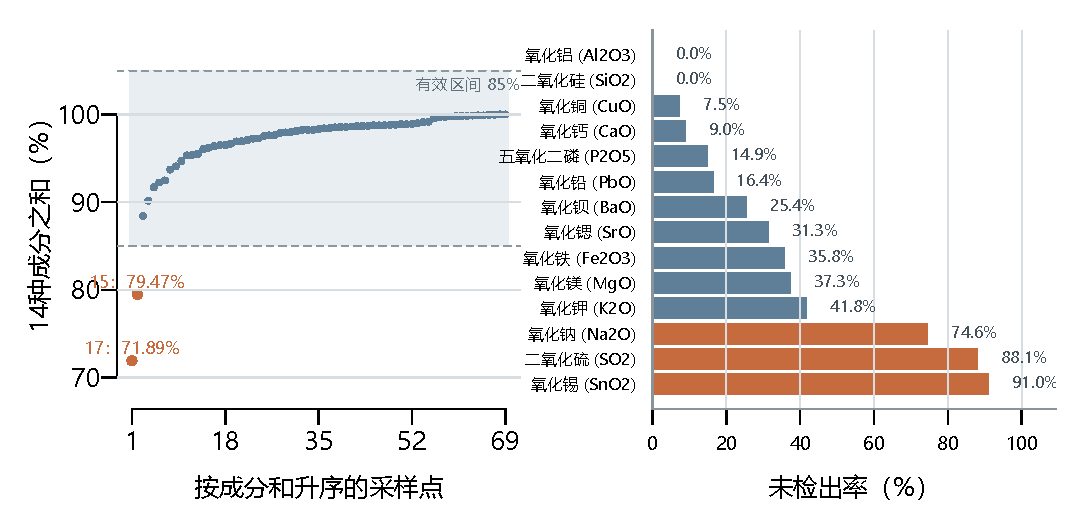
\includegraphics[width=0.96\textwidth]{figures/data_preprocess_diagnostics.pdf}
    \caption{成分和有效性与各成分未检出率组合诊断}
    \label{fig:data-diagnostics}
\end{figure}

\subsection{代表成分与颜色热卡填补}
仅为补全4件颜色缺失文物，按文物编号构造代表成分：单一采样点直接采用；两个普通部位取14种成分的算术平均；普通部位与严重风化点按\(1:2\)加权；普通部位与未风化点并存时采用普通部位；只有未风化点时取其均值。上述普通、未风化和严重风化状态均由完整采样点名称逐行判定；无效的15、17号成分不参与代表成分和供体距离计算。

对代表成分依次闭合、近零替换并作CLR变换，在CLR空间以欧氏距离计算Aitchison距离。供体限定为玻璃类型、纹饰均相同且颜色已知的文物，取最近5个供体按距离倒数投票；若获胜颜色票重占比不足50\%，则回退至同玻璃类型颜色众数。结果见表\ref{tab:color-imputation}；40号因票重不足而回退，且对近零参数较敏感，故问题一另以“使用填充值/排除4件缺色文物”作对照分析。

\begin{table}[H]
    \centering
    \caption{缺失颜色的文物级填补结果（\(\delta=0.02\%\)）}
    \label{tab:color-imputation}
    \small
    \begin{tabular}{ccc}
        \toprule
        文物编号 & 最终颜色 & 处理方式 \\
        \midrule
        19 & 黑 & 热卡填补 \\
        40 & 浅蓝 & 票重不足50\%，同类型众数回退 \\
        48 & 浅蓝 & 热卡填补 \\
        58 & 浅蓝 & 热卡填补 \\
        \bottomrule
    \end{tabular}
\end{table}

\subsection{闭合、近零替换与CLR变换}
为消除记录总量偏离100\%造成的不可比性，先对每个有效采样点闭合：
\begin{equation}
    c_{irj}=100\frac{x_{irj}}{S_{ir}}.
    \label{eq:closure}
\end{equation}
有效训练数据的最小正成分为0.04\%，取其一半\(\delta=0.02\%\)。若一行有\(k\)个零值，则每个零替换为\(\delta\)，其余正成分统一乘以\((100-k\delta)/100\)，从而仍保持行和为100\%。在\(\delta=0.01\%,0.02\%,0.04\%\)下重复诊断，均未产生新增剔除点；相对\(0.02\%\)基准，供体集合分别有3、0、4处变化。颜色及供体对近零参数的完整变化由敏感性工作表记录，因此将颜色填补作为不确定性来源在问题一中作“保留填充值/剔除缺色文物”的对照，而不将其当作确定观测。

随后以中心对数比变换进入成分分析空间：
\begin{equation}
    z_{irj}=\ln\!\left(\frac{c_{irj}^{+}}
    {\left(\prod_{j=1}^{14}c_{irj}^{+}\right)^{1/14}}\right).
    \label{eq:clr}
\end{equation}
需要统一尺度的分类或聚类模型再取\(u_{irj}=(z_{irj}-\mu_j)/\sigma_j\)。\(\mu_j,\sigma_j\)仅由已分类训练集估计，表单3只套用表单2参数；交叉验证时以文物编号分组，并在每一训练折重新估计参数，以避免同一文物泄漏及标准化泄漏。图\ref{fig:data-flow}概括了该处理链。

\begin{figure}[H]
    \centering
    \begin{tikzpicture}[
        >=Latex,
        data/.style={draw=black!55, rounded corners=2pt, fill=blue!5, align=center, text width=3.25cm, minimum height=1.35cm, font=\small},
        process/.style={draw=black!55, rounded corners=2pt, fill=green!7, align=center, text width=3.45cm, minimum height=1.35cm, font=\small},
        output/.style={draw=black!55, rounded corners=2pt, fill=orange!9, align=center, text width=3.45cm, minimum height=1.35cm, font=\small},
        flow/.style={->, line width=.7pt, black!70}
    ]
        \node[data] (raw) {\textbf{原始数据层}\\表单1：58件文物\\表单2：69个采样点\\表单3：8个未知样品};
        \node[process, right=1.25cm of raw] (screen) {\textbf{有效性筛选}\\成分和\(\in[85,105]\%\)\\剔除15、17号化学成分\\得到67条有效采样点};
        \node[process, below=1.05cm of screen] (transform) {\textbf{成分数据变换}\\闭合归一化\(\rightarrow\)近零替换\\\(\delta=0.02\%\)\(\rightarrow\)CLR\(\rightarrow\)Z-score};
        \node[output, left=1.25cm of transform] (use) {\textbf{输出用途}\\颜色热卡填补与敏感性\\稳健异常诊断\\分类、聚类与未知样品变换};
        \draw[flow] (raw) -- (screen);
        \draw[flow] (screen) -- (transform);
        \draw[flow] (transform) -- (use);
    \end{tikzpicture}
    \caption{数据预处理流程与数据量变化}
    \label{fig:data-flow}
\end{figure}

\subsection{稳健异常诊断与使用规则}
按“玻璃类型\(\times\)二元采样点风化状态”分组，在CLR空间计算样本到分量中位数中心的Aitchison距离\(D_i\)。分别以
\begin{equation}
    T_{\mathrm{MAD}}=\operatorname{Med}(D)+3.5\operatorname{MAD}(D),\qquad
    T_{\mathrm{IQR}}=Q_3+1.5(Q_3-Q_1)
    \label{eq:robust-outlier}
\end{equation}
为阈值，仅同时超过二者时标记为稳健异常。除已按题目阈值剔除的15、17号外，未发现需删除的新增异常点；这避免把真实的严重风化特征误作测量错误。

最终，问题一至四使用67条有效采样点及其CLR/Z-CLR特征，表单3的8条记录使用同一套训练参数变换；58件文物属性仅用于关联、颜色补全和分组控制。MATLAB主程序从原始工作簿计算；R复核程序亦直接读取原始\texttt{question/附件.xlsx}，独立复算采样点状态、颜色填补、闭合、近零替换、CLR和稳健异常诊断，再与MATLAB关键CLR快照比对。完整供体距离、投票占比、异常阈值及中间数据见支撑工作簿\texttt{data/附件\_数据预处理结果.xlsx}。

\section{问题一：表面风化规律与风化前成分预测}

\subsection{风化与玻璃类型、纹饰和颜色的关系}

\subsubsection{列联表与独立性检验}
分别构造“风化状态—玻璃类型”“风化状态—纹饰”“风化状态—颜色”列联表。对于期望频数充分的列联表使用Pearson卡方检验；当存在较多小期望频数时，使用Fisher精确检验或Monte Carlo精确检验。

设列联表观测频数为\(O_{ab}\)，期望频数为\(E_{ab}\)，卡方统计量为
\begin{equation}
  \chi^2=\sum_a\sum_b\frac{(O_{ab}-E_{ab})^2}{E_{ab}}.
\end{equation}
检验原假设为“两个类别变量相互独立”。同时报告Cramér's \(V\)作为效应量，避免只依据\(p\)值判断关系强弱。

\subsubsection{二元逻辑回归}
为同时控制多种属性，建立风化概率模型：
\begin{equation}
  \log\frac{P(W_i=1)}{1-P(W_i=1)}
  =\beta_0+\beta_1T_i+\bm{\beta}_2^{\mathsf T}\bm{D}_{i,\mathrm{纹饰}}
  +\bm{\beta}_3^{\mathsf T}\bm{D}_{i,\mathrm{颜色}},
\end{equation}
其中分类变量采用哑变量编码。\todo{根据样本稀疏程度决定是否合并低频颜色，或采用Firth逻辑回归降低完全分离偏差。}

\subsection{分类型的风化成分统计规律}
分别在高钾玻璃和铅钡玻璃内部比较风化组与无风化组。对每种成分报告样本量、均值、标准差、中位数和四分位距。根据正态性、异常值及方差齐性检验选择独立样本\(t\)检验或Mann--Whitney \(U\)检验，并采用\todo{Benjamini--Hochberg等方法}控制14次重复检验的多重比较错误率。

定义第\(g\)类玻璃中成分\(j\)的风化变化比：
\begin{equation}
  q_{gj}=\frac{\operatorname{Med}(x_j\mid W=1,T=g)}
  {\operatorname{Med}(x_j\mid W=0,T=g)}.
\end{equation}
当\(q_{gj}>1\)时，表示该成分在比例意义上随风化相对升高；反之相对降低。需强调，该指标描述的是成分比例变化，而非元素绝对质量变化。

\subsection{风化前化学成分预测模型}

\subsubsection{基准比例恢复模型}
若配对样本有限，可先依据同类型风化组和无风化组的稳健中心构造恢复因子：
\begin{equation}
  a_{gj}=\frac{\operatorname{Med}(x_j\mid W=0,T=g)}
  {\operatorname{Med}(x_j\mid W=1,T=g)+\varepsilon},
\end{equation}
并对风化点进行初步恢复：
\begin{equation}
  \tilde{x}_{ij}^{(0)}=a_{g j}x_{ij}^{(w)},\qquad
  \hat{x}_{ij}^{(0)}=100\frac{\tilde{x}_{ij}^{(0)}}{\sum_k\tilde{x}_{ik}^{(0)}}.
\end{equation}
其中\(\varepsilon\)用于避免分母为0。

\subsubsection{候选回归模型}
若可构造足够可靠的配对或近似配对样本，则比较以下方案：
\begin{itemize}
  \item 分成分稳健线性回归；
  \item 偏最小二乘回归，缓解成分间共线性；
  \item 简单树模型作为非线性对照，但限制深度以防过拟合。
\end{itemize}
模型以按文物分组的交叉验证误差、成分和约束满足度及解释性为选择标准。

\subsection{结果与解释}
\todo{填入风化关联检验表、关键成分变化表、风化前预测结果表和误差指标。解释时区分“统计显著”“效应大小”“化学意义”三个层次。}

\section{问题二：玻璃类型判别与亚类划分}
\label{sec:problem2}

\subsection{建模口径与总体思路}
问题二关注的是已分类文物的成分规律，而不是对表单3未知文物作出最终归类；后者留在问题三处理。
因此，本文以表单2的67个有效采样点为分析单位，并将同一文物的多个采样点视为相关观测。
其中铅钡玻璃49点、高钾玻璃18点，来自56件文物。
为避免将同一文物的不同部位同时用于训练与验证，所有二分类性能均在按文物编号分组的5折验证中计算。

各成分已在数据预处理阶段闭合、近零替换并进行CLR变换，故本节不再重复处理零值或剔除异常值。
纹饰、颜色和整体风化状态不进入二分类器：玻璃类型本身是待解释标签，且这些辅助字段不能替代化学检测证据；本节只以14个CLR成分坐标建立可复核的化学判别规则。
模型链为“信息增益决策树给出规则---PLS--DA检验判别稳定性并排序变量重要性---分类型K-means进行亚类划分”。

\subsection{高钾与铅钡玻璃二分类}
\subsubsection{可解释决策规则}
设第$i$个采样点的CLR成分向量为$\bm z_i$，类别$T_i\in\{1,2\}$分别表示铅钡和高钾玻璃。
在节点样本集$D$上，连续变量$z_j$的候选阈值$t$按信息增益
\begin{equation}
    \operatorname{Gain}(D,z_j,t)=H(D)-\frac{|D_-|}{|D|}H(D_-)-\frac{|D_+|}{|D|}H(D_+)
\end{equation}
选择，其中$D_-=\{i:z_{ij}<t\}$、$D_+=D\setminus D_-$，且
\begin{equation}
    H(D)=-\sum_{g=1}^{2}p_g\log_2p_g.
\end{equation}
该准则直接对应于“尽量使分裂后节点类别更纯”的考古判别需求；相较于深层黑箱模型，浅层树还能给出可审计的阈值规则\cite{breiman1984}。

在全部67点上拟合并以分组验证选择剪枝参数后，最终树仅含一个分裂节点：
\begin{equation}
    \mathrm{clr}(\mathrm{PbO})<1.7497\ \Rightarrow\ \text{高钾玻璃},\qquad
    \mathrm{clr}(\mathrm{PbO})\geq1.7497\ \Rightarrow\ \text{铅钡玻璃}.
    \label{eq:p2-tree-rule}
\end{equation}
这里的阈值比较的是PbO相对于该点全部成分几何均值的对数比，并非PbO原始百分数阈值。
这与铅矿助熔使铅钡玻璃PbO相对丰度更高的工艺机理相符。
不过，树在训练集上的完全分离不能视作泛化性能；按文物分组的平衡准确率为0.8333，说明少数文物的点位仍会跨过该单变量边界。

\begin{figure}[H]
    \centering
    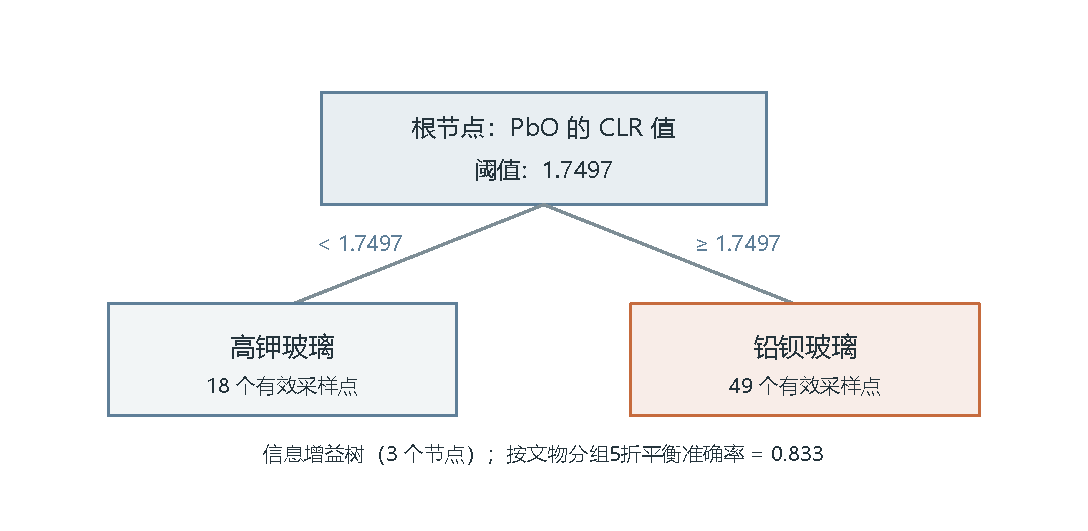
\includegraphics[width=0.82\textwidth]{figures/problem2_decision_tree.pdf}
    \caption{基于PbO的CLR可解释决策树}
    \label{fig:p2-decision-tree}
\end{figure}

\subsubsection{PLS--DA复核与重要成分}
为利用多成分的联合信息，将类别编码为两列哑变量矩阵$\bm Y$，并在训练折内对CLR坐标重新标准化。
偏最小二乘判别分析写为
\begin{equation}
    \bm X=\bm T\bm P^{\mathsf T}+\bm E_X,qquad
    \bm Y=\bm T\bm Q^{\mathsf T}+\bm E_Y,
    \label{eq:p2-plsda}
\end{equation}
其中潜变量$\bm T$同时解释成分矩阵$\bm X$和类别矩阵$\bm Y$。
在候选的1--5个潜变量中，1个潜变量取得最高的分组验证性能，故不继续增加自由度。
变量$j$的重要性按
\begin{equation}
    \operatorname{VIP}_{j}=\sqrt{14\cdot
    \frac{\sum_{a}\operatorname{SSY}_{a}w_{ja}^{2}}
    {\sum_{a}\operatorname{SSY}_{a}}}
    \label{eq:p2-vip}
\end{equation}
计算；其中$w_{ja}$为第$a$个潜变量的标准化权重，$\operatorname{SSY}_a$为该潜变量解释的类别平方和\cite{wold2001}。

\begin{table}[H]
    \centering
    \caption{两类玻璃判别的按文物分组验证结果}
    \label{tab:p2-binary-validation}
    \small
    \begin{tabular}{lccc}
        \toprule
        方法 & 潜变量数/树节点数 & 准确率 & 平衡准确率 / 宏平均F1 \\
        \midrule
        信息增益决策树 & 3个节点 & 0.9104 & 0.8333 / 0.8712 \\
        PLS--DA & 1个潜变量 & 0.9851 & 0.9722 / 0.9807 \\
        \bottomrule
    \end{tabular}
\end{table}

表\ref{tab:p2-binary-validation}表明，单一PbO相对丰度已经提供了直观的初筛规则，而一维PLS--DA利用其他成分后对不同文物的迁移更稳定。
因此，式\eqref{eq:p2-tree-rule}用于解释分类机理，PLS--DA作为后续未知样品判别的主要化学评分器；PLS--DA的输出是判别得分，不能误称为已校准概率。

\begin{figure}[H]
    \centering
    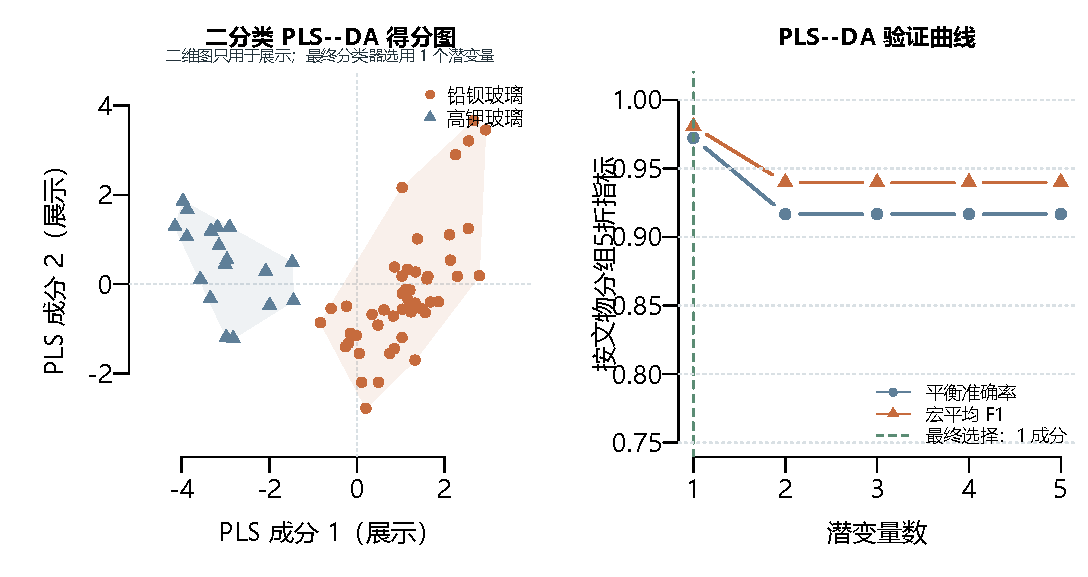
\includegraphics[width=\textwidth]{figures/problem2_binary_plsda.pdf}
    \caption{二分类PLS--DA二维展示与按文物分组验证曲线}
    \label{fig:p2-binary-plsda}
\end{figure}

\begin{table}[H]
    \centering
    \caption{二分类中VIP大于1的化学成分}
    \label{tab:p2-binary-vip}
    \small
    \begin{tabular}{ccccccc}
        \toprule
        排名 & 1 & 2 & 3 & 4 & 5 & 6 \\
        \midrule
        成分 & PbO & BaO & K$_2$O & SiO$_2$ & SrO & Al$_2$O$_3$ \\
        VIP & 1.915 & 1.566 & 1.505 & 1.193 & 1.109 & 1.100 \\
        \bottomrule
    \end{tabular}
\end{table}

PbO、BaO和K$_2$O分别对应铅钡助熔和草木灰助熔的主要差异，位居前三具有明确工艺解释；SiO$_2$、SrO和Al$_2$O$_3$补充刻画了基质与伴生矿物差异。
其余8种成分的VIP均不大于1，故不将它们作为两类玻璃的主要判别证据。

\subsection{分类型的亚类划分}
\subsubsection{特征与聚类数选择}
若直接在全部14个CLR坐标上聚类，低变异坐标会放大测量噪声且CLR坐标存在一条线性约束。
因此，对每个大类分别按组内CLR中位数绝对偏差（MAD）排序，保留变异最大的5个坐标，再在其组内标准化空间中求解K-means目标函数
\begin{equation}
    J_K=\sum_{g=1}^{K}\sum_{i\in C_g}\lVert\bm u_i-\bm\mu_g\rVert_2^2,
    \label{eq:p2-kmeans}
\end{equation}
其中$\bm u_i$为选定CLR坐标的标准化向量。
K-means以固定随机种子和100次随机起点运行；类别编号仅是按第一入模坐标中心排序的记号，不赋予年代或产地含义\cite{macqueen1967}。

聚类数不能只凭肘部图决定，本文同时要求每个最终簇至少含3个点，并检查平均轮廓系数、初始化稳定性和特征替换敏感性。
结果如表\ref{tab:p2-cluster-choice}：高钾组在$K=4$时的轮廓系数为0.660，且$K=5$开始出现单点簇；铅钡组从$K=4$到$K=5$的轮廓系数由0.292升至0.327，5簇的最小规模仍为8，故保留$K=5$。

\begin{table}[H]
    \centering
    \caption{两类玻璃的亚类划分设置与结果}
    \label{tab:p2-cluster-choice}
    \small
    \begin{tabularx}{\textwidth}{lXcS[table-format=3.3]S[table-format=1.3]c}
        \toprule
        玻璃类型 & 入模CLR成分（按组内MAD前五） & $K$ & {组内平方和} & {平均轮廓系数} & 簇规模 \\
        \midrule
        高钾 & PbO、BaO、Na$_2$O、SiO$_2$、SO$_2$ & 4 & 11.274 & 0.660 & 3, 8, 3, 4 \\
        铅钡 & Fe$_2$O$_3$、P$_2$O$_5$、K$_2$O、MgO、CuO & 5 & 91.937 & 0.327 & 11, 10, 11, 8, 9 \\
        \bottomrule
    \end{tabularx}
\end{table}

表\ref{tab:p2-cluster-choice}中的特征集合是各大类内部差异最大的成分，并不等价于表\ref{tab:p2-binary-vip}中区分两大类的成分。
图\ref{fig:p2-k-selection}同时呈现肘部下降和轮廓诊断：轮廓系数只作为检验分离度的辅助证据，不替代最小簇规模与稳定性约束。

\begin{figure}[H]
    \centering
    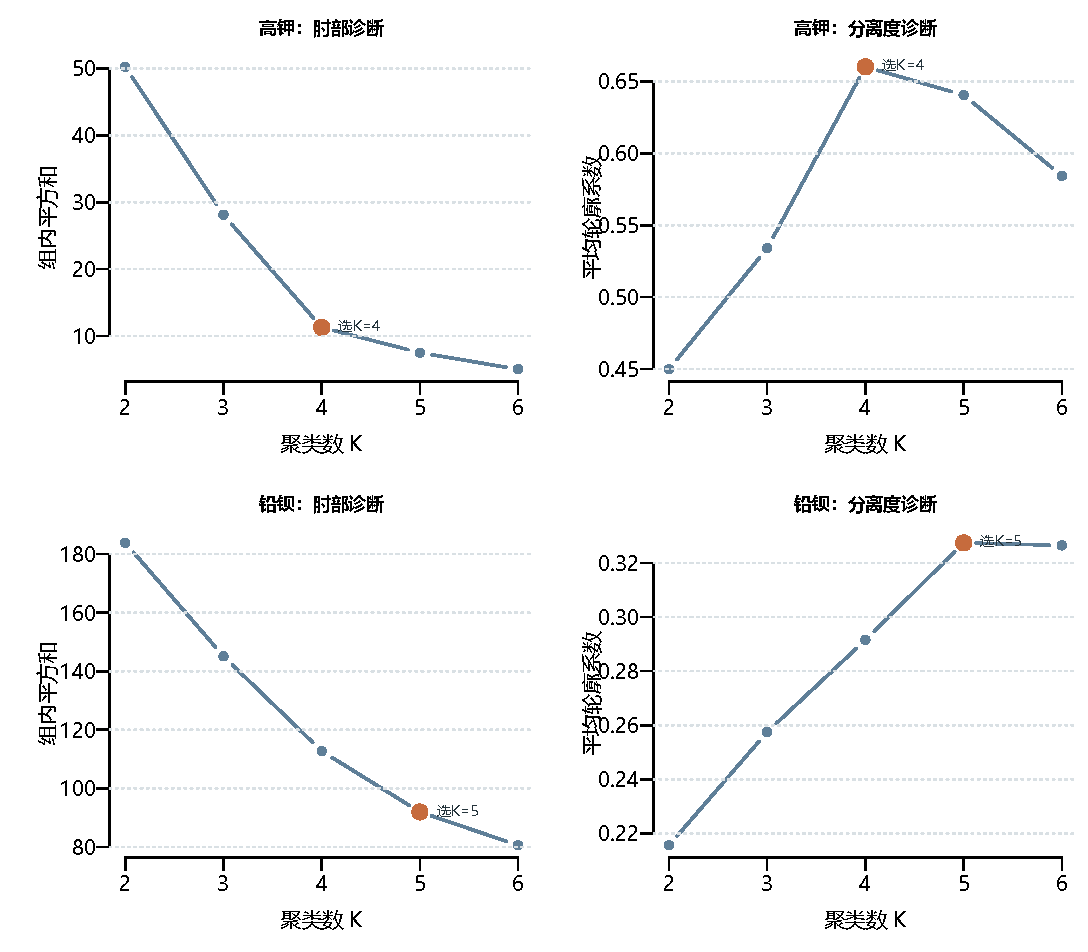
\includegraphics[width=0.90\textwidth]{figures/problem2_kmeans_selection.pdf}
    \caption{高钾与铅钡玻璃的K-means聚类数诊断}
    \label{fig:p2-k-selection}
\end{figure}

\begin{figure}[H]
    \centering
    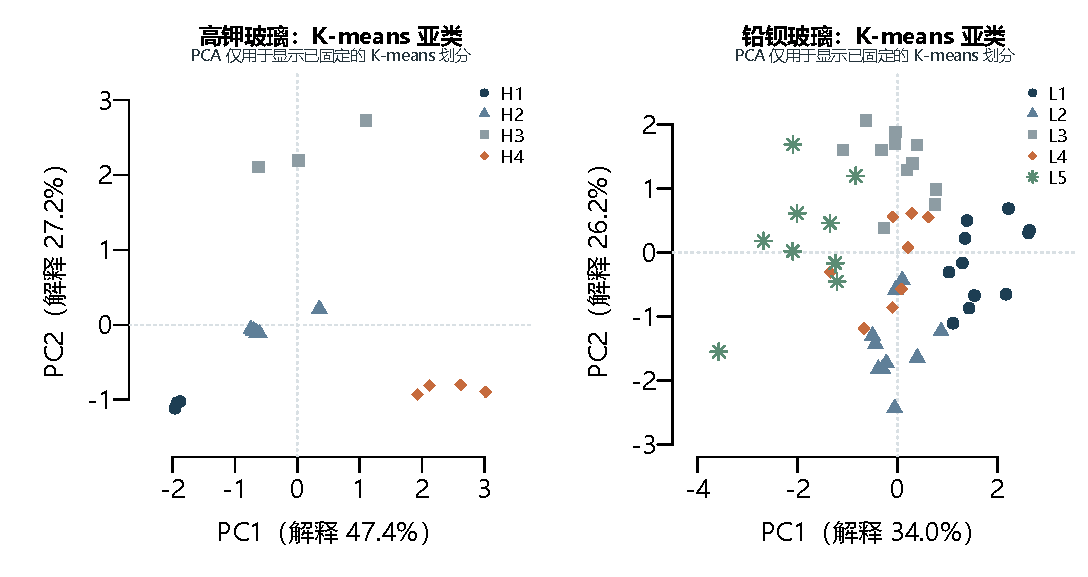
\includegraphics[width=\textwidth]{figures/problem2_kmeans_clusters.pdf}
    \caption{两类玻璃的K-means亚类在二维PCA投影中的显示}
    \label{fig:p2-kmeans-clusters}
\end{figure}

图\ref{fig:p2-kmeans-clusters}中的PCA仅将已确定的五维聚类空间投影到二维，坐标并未参与K-means的分配；因此二维重叠不改变表\ref{tab:p2-cluster-choice}中的高维聚类结论。
高钾玻璃的四个采样点亚类依次为：
\(\{01,04,05\}\)、
\(\{03\text{部位}1,07,09,10,12,18,22,27\}\)、
\(\{13,14,16\}\)和
\(\{03\text{部位}2,06\text{部位}1,06\text{部位}2,21\}\)。
铅钡玻璃五个亚类的完整采样点清单、全部14维中心及二次PLS--DA的VIP排序另存于支持材料，避免在正文中把长名单误排为文物级结论。

\subsubsection{亚类中心的成分特征}
聚类中心先在CLR空间取均值，再以逆CLR变换为和为$100\%$的组成；故表中的数值是近零替换口径下的几何中心，而不是各原始比例的算术平均。

\begin{table}[H]
    \centering
    \caption{高钾玻璃亚类的CLR逆变换中心（\%）}
    \label{tab:p2-high-centers}
    \small
    \begin{tabular}{ccccccc}
        \toprule
        亚类 & 样本数 & SiO$_2$ & K$_2$O & PbO & BaO & SO$_2$ \\
        \midrule
        H1 & 3 & 68.03 & 10.58 & 0.02 & 0.02 & 0.42 \\
        H2 & 8 & 95.26 & 0.57 & 0.03 & 0.02 & 0.02 \\
        H3 & 3 & 64.63 & 13.59 & 0.16 & 0.02 & 0.02 \\
        H4 & 4 & 74.29 & 2.17 & 0.63 & 1.86 & 0.02 \\
        \bottomrule
    \end{tabular}
\end{table}

H1与H3均表现为较高K$_2$O和较低SiO$_2$，但H3的Na$_2$O中心为$2.84\%$，高于H1的$0.02\%$；H2以高SiO$_2$为主；H4则具有相对较高的PbO和BaO。
这说明高钾玻璃内部并非单一配方，但小簇H1和H3各仅含3点，应理解为待进一步考古材料验证的组成型，而非确定的工艺谱系。

\begin{table}[H]
    \centering
    \caption{铅钡玻璃亚类的CLR逆变换中心（\%）}
    \label{tab:p2-lead-centers}
    \small
    \begin{tabular}{ccccccccc}
        \toprule
        亚类 & 样本数 & SiO$_2$ & MgO & Fe$_2$O$_3$ & CuO & PbO & BaO & P$_2$O$_5$ \\
        \midrule
        L1 & 11 & 26.94 & 0.03 & 0.02 & 3.62 & 40.68 & 22.78 & 1.65 \\
        L2 & 10 & 53.14 & 1.17 & 0.03 & 1.43 & 28.10 & 10.21 & 0.08 \\
        L3 & 11 & 32.60 & 1.00 & 0.56 & 1.34 & 46.29 & 2.64 & 8.87 \\
        L4 & 8 & 54.92 & 0.02 & 0.68 & 0.75 & 29.45 & 9.74 & 0.30 \\
        L5 & 9 & 46.73 & 0.93 & 1.28 & 0.12 & 35.90 & 3.90 & 1.36 \\
        \bottomrule
    \end{tabular}
\end{table}

铅钡亚类的差异主要体现在PbO--BaO组合以及Fe$_2$O$_3$、P$_2$O$_5$和CuO的伴生含量：L1具有较高PbO和BaO，L3的PbO和P$_2$O$_5$中心最高，而L5的Fe$_2$O$_3$中心最高、CuO中心最低。
与此一致，亚类PLS--DA的VIP前五项为MgO、CuO、Fe$_2$O$_3$、P$_2$O$_5$和K$_2$O；高钾亚类的VIP前五项为SiO$_2$、SO$_2$、Na$_2$O、BaO和SnO$_2$。
这些VIP仅描述已获得聚类标签后的分离方向，不能反过来证明聚类为唯一真值。

\begin{figure}[H]
    \centering
    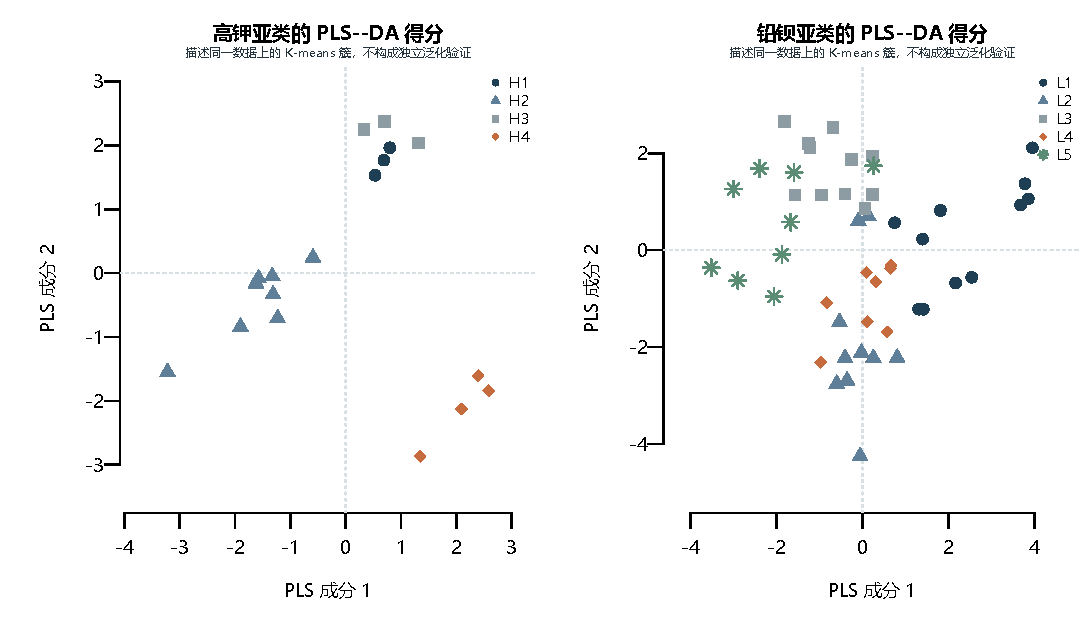
\includegraphics[width=\textwidth]{figures/problem2_subclass_plsda.pdf}
    \caption{两类玻璃亚类的PLS--DA描述性得分图}
    \label{fig:p2-subclass-plsda}
\end{figure}

图\ref{fig:p2-subclass-plsda}以K-means得到的同一批标签构造，故用于呈现各亚类在成分潜变量上的分离方向，不将图中的分离程度报告为独立测试集准确率。

\subsection{合理性与敏感性分析}
聚类结果的敏感性以调整兰德指数（ARI）衡量；ARI为1表示两次划分完全一致。
对高钾玻璃，标准化CLR坐标加入标准差0.03的独立噪声后，100次重算的ARI均为1；铅钡玻璃的平均ARI为0.998，最小值为0.944。
因此，已选成分的小幅测量扰动不会实质改变两类玻璃的亚类归属。

随机初始化则暴露出K-means的局部最优风险：100次单起点运行中，高钾和铅钡的平均ARI分别为0.874和0.889，最小值分别为0.537和0.421。
这正是最终计算固定种子并采用100次起点的原因，而不是将某一次随机运行当作结论。
特征筛选方面，高钾组将前五变量缩为前四或扩展为前六时ARI均为1；铅钡组对应ARI为0.668和0.893，说明其细分结构更依赖对Fe$_2$O$_3$、P$_2$O$_5$、K$_2$O、MgO和CuO的联合刻画。

\begin{figure}[H]
    \centering
    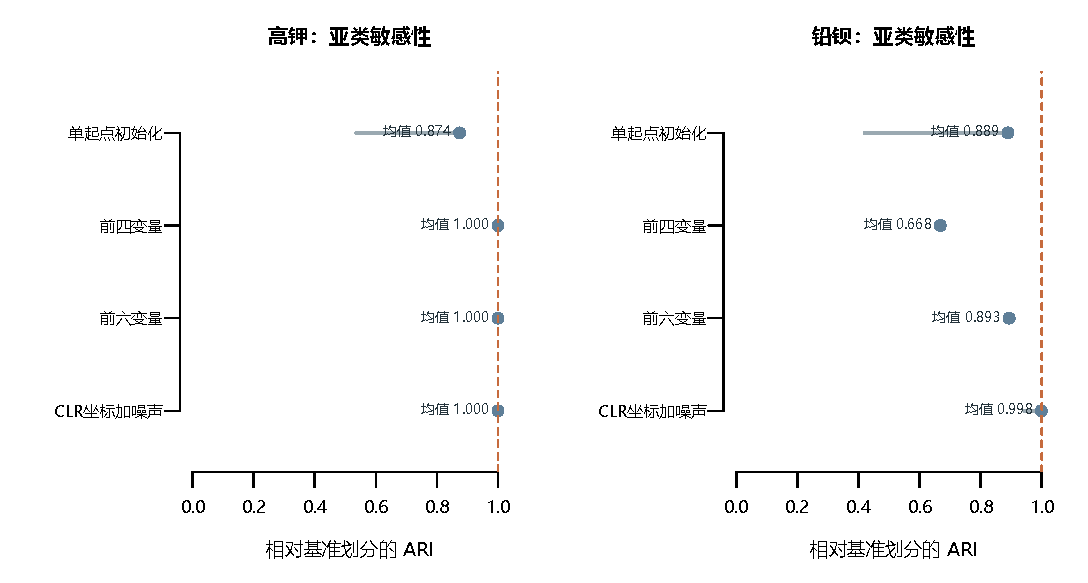
\includegraphics[width=\textwidth]{figures/problem2_kmeans_sensitivity.pdf}
    \caption{两类玻璃亚类的初始化、特征组合与小扰动敏感性}
    \label{fig:p2-kmeans-sensitivity}
\end{figure}

综上，二类玻璃的主判别规律稳健地指向PbO、BaO和K$_2$O等助熔相关成分；高钾的4个亚类对小扰动稳定但受样本量限制，铅钡的5个亚类具有中等轮廓分离度且对特征筛选更敏感。
亚类划分应作为后续样品比较与问题三敏感性分析的组成参照，而不应直接等同于独立的考古类型。

\section{问题三：未知类别玻璃的鉴别}

\subsection{未知样品预处理}
对表单3执行与训练数据完全一致的有效性检验、零值替代、闭合归一化、变量变换和标准化。所有预处理参数仅由已分类训练样本估计，再应用于A1--A8，避免使用未知样品信息反向影响模型。

\subsection{类别预测}
将未知样品输入问题二选定的分类器，输出预测类别、类别概率或判别距离。

\begin{table}[H]
  \centering
  \caption{未知样品类别鉴别结果}
  \label{tab:unknown-result}
  \small
  \begin{tabularx}{\textwidth}{C{1.2cm} C{2.2cm} C{2.2cm} Y C{2.0cm}}
    \toprule
    样品 & 风化状态 & 预测类型 & 属于铅钡的概率或判别得分 & 稳定性 \\
    \midrule
    A1 & \todo{填写} & \todo{填写} & \todo{填写} & \todo{填写} \\
    A2 & \todo{填写} & \todo{填写} & \todo{填写} & \todo{填写} \\
    A3 & \todo{填写} & \todo{填写} & \todo{填写} & \todo{填写} \\
    A4 & \todo{填写} & \todo{填写} & \todo{填写} & \todo{填写} \\
    A5 & \todo{填写} & \todo{填写} & \todo{填写} & \todo{填写} \\
    A6 & \todo{填写} & \todo{填写} & \todo{填写} & \todo{填写} \\
    A7 & \todo{填写} & \todo{填写} & \todo{填写} & \todo{填写} \\
    A8 & \todo{填写} & \todo{填写} & \todo{填写} & \todo{填写} \\
    \bottomrule
  \end{tabularx}
\end{table}

\subsection{分类敏感性分析}
对每个未知样品的成分进行多次小幅扰动，并在每次扰动后重新执行完整预处理与分类。定义样品\(i\)的稳定率为
\begin{equation}
  S_i=\frac{1}{B}\sum_{b=1}^{B}
  I\!\left(\hat{T}_i^{(b)}=\hat{T}_i^{(0)}\right),
\end{equation}
其中\(B\)为扰动次数。若\(S_i\)较低或预测概率接近阈值，则将该样品标记为边界样品，并重点讨论其不确定性。

同时比较逻辑回归、LDA、决策树或SVM等候选模型对A1--A8的预测一致性。\todo{列出发生分歧的样品及原因。}

\section{问题四：化学成分关联关系及类别差异}

\subsection{成分数据的闭合效应}
由于14种成分之和接近\(100\%\)，一个成分比例上升会被动压缩其他成分比例，直接相关分析可能产生伪相关。因此，在零值替代和闭合归一化后，优先使用中心化对数比变换：
\begin{equation}
  \operatorname{clr}(c_{ij})
  =\ln\frac{c_{ij}}{g(\bm{c}_i)},\qquad
  g(\bm{c}_i)=\left(\prod_{j=1}^{D}c_{ij}\right)^{1/D}.
\end{equation}

\subsection{分类型关联分析}
分别对高钾玻璃和铅钡玻璃计算CLR变量之间的Pearson相关系数，并以Spearman相关系数作为稳健性对照。对检出率极低或近零方差成分不进行强行解释。

\begin{figure}[H]
  \centering
  \begin{subfigure}{0.47\textwidth}
    \centering
    \fbox{\parbox[c][5.0cm][c]{0.9\linewidth}{\centering\todo{高钾玻璃相关热力图}}}
    \caption{高钾玻璃}
  \end{subfigure}
  \hfill
  \begin{subfigure}{0.47\textwidth}
    \centering
    \fbox{\parbox[c][5.0cm][c]{0.9\linewidth}{\centering\todo{铅钡玻璃相关热力图}}}
    \caption{铅钡玻璃}
  \end{subfigure}
  \caption{不同玻璃类型的成分关联结构}
  \label{fig:corr-heatmap}
\end{figure}

\subsection{两类玻璃关联差异比较}
对每对成分\((j,k)\)，定义相关差异
\begin{equation}
  \Delta r_{jk}=r_{jk}^{(\mathrm{高钾})}-r_{jk}^{(\mathrm{铅钡})}.
\end{equation}
通过Fisher \(z\)变换或自助法构造差异置信区间，筛选在两类玻璃中方向相反或强度差异显著的成分对。重点报告少量稳定且具有配方或风化解释的关联，而不是机械罗列全部\(91\)组成分对。

\subsection{结果解释}
\todo{总结两类玻璃最强的正、负关联；列出差异最大的成分对；结合助熔剂、稳定剂及风化过程解释差异，同时明确相关关系不等于因果关系。}

\section{模型检验与稳健性分析}

\subsection{分类模型检验}
采用按文物编号分组的分层交叉验证，保证同一文物的多个采样点不会同时出现在训练集和测试集中。报告混淆矩阵、平衡准确率、宏平均F1值、灵敏度、特异度及ROC--AUC。

\subsection{恢复模型检验}
若存在可用的未风化点或模拟留出样本，则报告平均绝对误差、均方根误差及成分和偏差：
\begin{align}
  \mathrm{MAE} &= \frac{1}{nD}\sum_{i=1}^n\sum_{j=1}^D
  \left|x_{ij}^{(0)}-\hat{x}_{ij}^{(0)}\right|,\\
  \mathrm{RMSE} &= \sqrt{\frac{1}{nD}\sum_{i=1}^n\sum_{j=1}^D
  \left(x_{ij}^{(0)}-\hat{x}_{ij}^{(0)}\right)^2}.
\end{align}
同时检查恢复后各成分是否非负、总和是否接近\(100\%\)。

\subsection{关键假设敏感性}
至少比较以下设定：
\begin{enumerate}
  \item 有效样本阈值和归一化方法；
  \item 零值替代量；
  \item 是否合并同一文物的普通部位；
  \item 是否对风化样品先恢复再分类；
  \item 分类器、聚类算法和聚类数；
  \item 输入成分的随机扰动幅度。
\end{enumerate}

\subsection{误差来源}
\todo{分析检测误差、未观测埋藏环境、样本量小、类别不平衡、风化点配对不足及成分闭合约束等误差来源。}

\section{模型评价与结论}

\subsection{模型优点}
\begin{enumerate}
  \item 建模链条与四个问题一一对应，避免使用与题目目标无关的评价、优化或时间序列模型。
  \item 同时考虑无效数据、未检出值、重复采样和成分闭合效应，数据处理较为完整。
  \item 分类模型优先选择低复杂度、可解释方法，并以按文物分组的交叉验证降低信息泄漏。
  \item 对未知样品和亚类划分均进行扰动敏感性分析，不只给出单一确定结论。
\end{enumerate}

\subsection{模型局限}
\begin{enumerate}
  \item 缺少充足的同一文物风化点—未风化点配对数据，风化前成分恢复主要依赖横截面规律，因果解释有限。
  \item 埋藏时间、环境酸碱度和温湿度等变量未被观测，可能形成遗漏变量偏差。
  \item 部分微量成分未检出比例较高，其相关关系和聚类贡献存在不确定性。
\end{enumerate}

\subsection{主要结论}
\begin{enumerate}
  \item \todo{问题一结论：风化与哪些属性显著相关，关键成分如何变化，恢复模型误差如何。}
  \item \todo{问题二结论：高钾/铅钡的核心分类规律，各自划分为哪些亚类。}
  \item \todo{问题三结论：A1--A8的类型及边界样品。}
  \item \todo{问题四结论：两类玻璃的主要成分关联及差异。}
\end{enumerate}

\begin{thebibliography}{99}
  \bibitem{aitchison1986}
  Aitchison J. \textit{The Statistical Analysis of Compositional Data}[M]. London: Chapman and Hall, 1986.

  \bibitem{fisher1921}
  Fisher R A. On the probable error of a coefficient of correlation deduced from a small sample[J]. Metron, 1921, 1: 3--32.

  \bibitem{breiman1984}
  Breiman L, Friedman J H, Olshen R A, Stone C J. \textit{Classification and Regression Trees}[M]. Belmont: Wadsworth, 1984.

  \bibitem{wold2001}
  Wold S, Sj\"ostrom M, Eriksson L. PLS-regression: a basic tool of chemometrics[J]. Chemometrics and Intelligent Laboratory Systems, 2001, 58(2): 109--130.

  \bibitem{macqueen1967}
  MacQueen J B. Some methods for classification and analysis of multivariate observations[C]//Proceedings of the Fifth Berkeley Symposium on Mathematical Statistics and Probability. Berkeley: University of California Press, 1967: 281--297.

  \bibitem{sklearn}
  \todo{补充实际使用的软件、算法文献和自主查阅数据来源；正文引用处应使用\texttt{\textbackslash cite\{\}}标注。}
\end{thebibliography}


% 2022年格式规范未强制要求AI声明；若当届或赛区另有要求，再取消下行注释。
% \section*{生成式人工智能工具使用说明}
\todo{仅在当届竞赛或赛区明确要求时保留。说明工具名称、使用环节、人工核验方式，不得包含参赛者身份信息。}


\appendix
\section{支持材料文件列表}

依据竞赛格式规范，附录列明支持材料文件，并提交全部完整、可运行的源程序。数据预处理采用 MATLAB R2025b 主计算、R 4.6.1 从原始XLSX独立复核；Python 检查工作簿结构并将统计图PDF渲染为PNG进行非空与尺寸验收。

\begin{longtable}{C{1.2cm} L{5.2cm} L{7.0cm}}
  \caption{支持材料文件列表}\label{tab:support-files}\\
  \toprule
  序号 & 文件名 & 内容说明 \\
  \midrule
  \endfirsthead
  \multicolumn{3}{c}{表\thetable\ （续）}\\
  \toprule
  序号 & 文件名 & 内容说明 \\
  \midrule
  \endhead
  1 & \texttt{code/preprocess.m} & 唯一MATLAB主程序：有效性筛选、颜色填补、闭合、近零替换、CLR、异常诊断及数据输出 \\
  2 & \texttt{code/verify\_preprocess.R} & R从原始XLSX独立读取并复算采样点状态、颜色填补、CLR、异常诊断与敏感性，再比对MATLAB CLR快照 \\
  3 & \texttt{code/make\_figures.R} & 仅读取清洗后的CSV快照，生成中文矢量PDF及300 dpi预览PNG \\
  4 & \texttt{code/verify\_outputs.py} & XLSX工作表结构检查及PDF渲染、尺寸、非空检查，不参与数值计算 \\
  5 & \texttt{data/附件\_数据预处理结果.xlsx} & 清洗记录、颜色填补、CLR及异常诊断等完整中间数据 \\
  6 & \texttt{data/verification\_snapshots/} & MATLAB读取原始工作簿后导出的三份CSV核验快照及关键结果快照 \\
  7 & \texttt{data/matlab\_preprocess\_summary.txt} & MATLAB运行摘要与样本计数日志 \\
  8 & \texttt{data/r\_preprocess\_consistency\_report.txt} & R与MATLAB数值一致性报告 \\
  9 & \texttt{figures/data\_preprocess\_diagnostics.pdf} & 中文矢量的成分和有效性与未检出率组合诊断图 \\
  10 & \texttt{figures/data\_preprocess\_diagnostics.png} & 组合诊断图的300 dpi预览图 \\
  11 & \texttt{data/*\_report.txt} & MATLAB、R、作图和PDF渲染的可复现运行报告 \\
  \bottomrule
\end{longtable}

\section{完整程序代码}
电子论文附录中可根据篇幅列出核心代码，完整可运行代码必须随支持材料提交，且不得包含学校、姓名、学号、赛区等身份信息。

\subsection{数据预处理程序}
完整主程序源代码见\texttt{code/preprocess.m}；独立复核程序见\texttt{code/verify\_preprocess.R}；图形脚本见\texttt{code/make\_figures.R}；工作簿与图形渲染检查程序见\texttt{code/verify\_outputs.py}。源程序与结果工作簿共同提交，不在正文重复粘贴。

\subsection{各问题求解程序}
问题一至问题四的求解程序在其完成后另列入本表，并与相应的输入、输出和运行说明一并提交。


\end{document}
